\documentclass[12pt]{article}
\usepackage[T1]{fontenc}
\usepackage{calc}
\usepackage{setspace}
\usepackage{multicol}
\usepackage{fancyheadings}
 
\usepackage{graphicx}
\usepackage{color}
\usepackage{rotating}
\usepackage{harvard}
\usepackage{aer}
\usepackage{aertt}
\usepackage{verbatim}
\usepackage{array}
\usepackage{multirow}

\setlength{\voffset}{-0.25in}
\setlength{\topmargin}{0pt}
\setlength{\hoffset}{0pt}
\setlength{\oddsidemargin}{0pt}
\setlength{\headheight}{0pt}
\setlength{\headsep}{.4in}
\setlength{\marginparsep}{0pt}
\setlength{\marginparwidth}{0pt}
\setlength{\marginparpush}{0pt}
\setlength{\footskip}{.1in}
\setlength{\textwidth}{6.5in}
\setlength{\textheight}{9.25in}
\setlength{\parskip}{0pc}

\renewcommand{\baselinestretch}{1.5}

\newcommand{\bi}{\begin{itemize}}
\newcommand{\ei}{\end{itemize}}
\newcommand{\be}{\begin{enumerate}}
\newcommand{\ee}{\end{enumerate}}
\newcommand{\bd}{\begin{description}}
\newcommand{\ed}{\end{description}}
\newcommand{\prbf}[1]{\textbf{#1}}
\newcommand{\prit}[1]{\textit{#1}}
\newcommand{\beq}{\begin{equation}}
\newcommand{\eeq}{\end{equation}}
\newcommand{\bdm}{\begin{displaymath}}
\newcommand{\edm}{\end{displaymath}}
\newcommand{\script}[1]{\begin{cal}#1\end{cal}}
\newcommand{\citee}[1]{\citename{#1} (\citeyear{#1})}
\newcommand{\h}[1]{\hat{#1}}
\newcommand{\ds}{\displaystyle}
\newcommand{\normal}{\mathcal{N}}
\newcommand{\app}
{
\appendix
}

%\newcommand{\appsection}[1]
%{
%\let\oldthesection\thesection
%\renewcommand{\thesection}{Appendix \oldthesection}
%\section{#1}\let\thesection\oldthesection
%\renewcommand{\theequation}{\thesection\arabic{equation}}
%\setcounter{equation}{0}
%}

\newcommand{\appsection}[1]
{
\section{#1}
\renewcommand{\theequation}{\thesection\arabic{equation}}
\setcounter{equation}{0}
}


%\pagestyle{empty}
\pagestyle{fancyplain}
\lhead{}
\chead{Regime Switching and Wages in Major League Baseball}
\rhead{\thepage}
\lfoot{}
\cfoot{}
\rfoot{}

\begin{document}

\section{Introduction}\label{s:intro}
Major League Baseball (MLB) players are among the highest paid workers in the American economy.  Their minimum salaries are several times that of the average American salary, and the average wages are an even greater multiple.  They enjoy a minimum salary of \$400,000 per year, an average salary exceeding \$2 million per year, guaranteed contracts, and arguably the strongest union in American history.  Stories of the financial escapades of professional baseball teams and the salaries they pay their employees are common in the sports and business press.

It was not always this way however.  It was not until the mid 1970s when professional baseball players blazed the trail for all professional athletes by gaining the right to bargain competitively for their wages.  Before that time, the reserve clause meant players were bound to their original employer for the duration of their careers.  The labor market for ballplayers was a classic monopsony.  Furthermore, players typically had a very low opportunity cost to play in MLB; most had little schooling and the only opportunities were outside of professional sports.  

So what determines the salary of a player in such an environment?  Market pressures surely did not force owners to pay players salaries commensurate with their marginal revenue product.  A seminal work by \citee{scully1974} finds a significant degree of monopsonistic exploitation of players during this time.  However, neither were players all paid the same salary, despite their opportunity costs being very similar.  Evidence suggests that salaries were not simply raised on an annual basis for all players at steady rates,\footnote{See \citee{haupert2009} for a discussion of MLB wages during different labor regimes.} and even a casual look at players salaries reveals that higher performing players were often more highly paid.  

It's possible then that subtle market forces tied salaries to productivity even though competition was severely restricted, but there is no reason to think this relationship remained constant for the near century that the reserve clause bound all players to one employer.  For example, during this time there were two world wars and a Great Depression that impacted both the supply of players and the demand among fans for professional sports, all of which can change the subtle forces that influence players', albeit limited, negotiating power.  It's also possible that performance characteristics, beyond wins and losses, appealed to fans and that this appeal evolved over the decades. 

The purpose of this paper is to estimate how experience and productivity influenced salaries during the period of the reserve clause, paying careful attention to how this relationship changed over time.  We have a unique and extensive dataset that includes player data on salary and productivity (performance statistics) for over 400 players for over 60 years (1911 through 1973).  All the previous literature concerning baseball salaries has been limited to data from one to five years, and only rarely have datasets on this topic covered as many as ten years.\footnote{Section \ref{s:lit} has a more detailed discussion of this literature.}  Indeed, such a long panel including reliable measures of worker productivity, precise salaries, and experience is rare even in the labor economics literature as a whole.  The long panel allows us to answer an important question that to date has been difficult to impossible to address: Can changes in the relationship between performance and salary be identified over time?  If so, this signals subtle changes in bargaining power or market forces during the reserve clause that would not otherwise be directly observable.

To answer this question we employ a Markov-regime-switching regression procedure, where each regression coefficient can switch between two or more values (i.e. switch regimes) as time progresses.  A regime is defined by a particular set of regression coefficients, so the regression line that explains the relationship between the dependent and explanatory variables can change as time goes on.  The procedure allows for only a fixed number of regimes, but has the flexibility to allow any number of switches between the regimes.  A regime change affects all players at the same time, so a change in a coefficient on a performance variable (where salary is the dependent variable) would indicate owners put a higher value on performance and pay their players accordingly, or that players hold more bargaining power and are more capable of attracting higher salaries for good performance.  The exogenous nature of the switching allows switching to occur for unknown or unmeasurable reasons and it is a change in the relationship of the dependent variable and independent variables that triggers the identification of such a switch.  For simplicity of interpretation and computational tractability, we assume the possibility of only two regimes which allows us to identify periods where players have relatively weak bargaining power versus periods with relatively strong bargaining power.  We identify the period between the Great Depression and the end of World War II as a period in which players had a higher average pay and were more highly paid for good performance.

\section{Historical Background}\label{s:history}
From its earliest days, Major League Baseball has been a monopsonistic employer.  Beginning in 1876 with the founding of the National League of Professional Base Ball Clubs (NL) the industry was designed such that employers (team owners) minimized the ability of employees (players) to sell their services competitively.  The name chosen for this new league was significant because up until this time, all baseball organizations had been player associations.  Now, as the name implied, players were to be employees of a club and members of a league.

The new league ``provided for a new order, ingeniously designed to be nourished on both monopoly and competition.  Under its aegis, member clubs were to compete with each other for renown and receipts, but only within the confines of a prescribed pattern.''\footnote{\citee{seymour}, page 85.}  Ultimately both stability and the disruption of bitter labor disputes would result from the formation of the National League.  Stability would bring about a superior brand of baseball, considered the best in the world.  Labor problems were key in the formation of competing leagues.\footnote{Failed competitors and their years of operation: Union Association 1884, American Association 1882-91, Players League 1890, Federal League 1914-15.  The American League was formed as a competing league in 1901 and merged with the National League in 1903.}  All of these failed, except the American League, which eventually partnered with the National League to form what is to today known as Major League Baseball.

For much of the first century after the formation of the National League the players had little say in any affairs of their clubs and no representation in the governing institutions of the League.  Club executives simply presented contracts to their players and refused to negotiate.  Clubs used a variety of measures to keep players in line, including sobriety regulations and medical examinations by club doctors and suspensions for poor play, illness or insubordination.  If a player violated any club directives, he could even be ``blacklisted'' from professional baseball until he repented.

Team owners formalized their control over the players with the adoption of the reserve clause following the 1879 season.  Owners agreed that each of them would ``reserve,'' or keep off the market, five players of their eleven man rosters for the following year.  The list of reserved players was circulated among all owners, and each agreed not to employ or even negotiate with any other team's reserved players.  The plan was initially designed to prevent rich teams from acquiring all the best players, or so they claimed.  Conveniently, it also created a monopsony labor market that owners could exploit.  The number of reserved players slowly increased over the years until entire club rosters were designated as reserved.  Beginning in 1887 the list became a clause in the standard player contract.  The reserve clause remained intact for nearly a century, turning the baseball labor market into a tightly controlled monopsony.

With baseball players bound to one employer in perpetuity by the reserve clause, the labor market for ballplayers was a classic monopsony.  Players were free to negotiate with prospective employers only for their first contract, usually as a young man, in many cases even a minor.  At this age the prospects for any player were extremely uncertain.  In addition, most unschooled young potential ballplayers lacked both the sophistication and the knowledge of the market to do much, if any, bargaining.  As a result, the first contract usually imparted little to the ballplayer in the way of bargaining leverage.  This began to change after World War II when the rules regarding bonus payments were liberalized, allowing some young players to receive hefty signing bonuses.  What did not change, however, was the presence of the reserve clause in the standard player contract.

Once signed to a professional contract, players lost control of their fate as a professional baseball player unless they were released from that contract at the discretion of the team.  The reserve clause gave teams the ability to renew a player's contract in perpetuity on terms dictated by the team.  The sale of contracts from one team to another was a common method of raising revenue for the sellers and building a better club for the buyers.  Consistent in all of this was the lack of any input by the player.  His only choice was to play for the new team or look for a job in a different line of work.

In this environment the only explicit leverage a player could exert was to threaten to hold out his services.  For most players this was not a realistic advantage, as the monopsony MLB held down the number of viable franchises in the league, and hence the number of employed ballplayers.  As a result, there were many players in lesser leagues scattered around the country who were viable substitutes for the player who held out his services.  A holdout strategy was only possible for the highest quality players at the peak of their career, for whom a viable substitute did not exist.  Even then, holdouts were rarely successful, as the opportunity cost of a holdout was much higher for the players than the teams.    

Joe DiMaggio, for example, staged a hold-out in the spring of 1938.  At the time he was arguably the best baseball player in the world.  He was a celebrity and a fan favorite with enormous drawing power.  If anybody should have been able to execute a successful holdout, it would have been Joe DiMaggio in 1938.  The Yankees were coming off back-to-back World Series championships and their highest attendance in seven years.  Not since Babe Ruth retired had the team done so well on or off the field.  For his contribution, DiMaggio had just put together two of the finest seasons in baseball history, and the fact that they were his first two seasons made this performance all the more remarkable.  Connie Mack, the venerable owner of the Philadelphia Athletics and a fifty year baseball veteran, called him the greatest drawing card in the game.  DiMaggio was a full-fledged superstar.

When he asked for a raise from \$15,000 to \$40,000 it seemed to him like a reasonable request.  In fact, his marginal revenue product (MRP) that year was approximately \$400,000, so even at \$40,000 the club would be getting a steal.\footnote{See \citee{haupert2009}.}  However, DiMaggio discovered that management was holding all the cards.  Not only was the reserve clause working against him, but so was the press, and as a result, the fans.

DiMaggio threatened to stage an indefinite holdout, but three days after the season started, he caved in.  Yankee owner Jacob Ruppert triumphantly shared his telegram with the press: ``Your terms accepted,'' adding that DiMaggio's salary would be docked each day until his manager deemed him ready to play.  That turned out to be nearly two weeks and almost \$1500 into the season.  Perhaps worse than the lost salary was the lost adulation of the fans, who had been turned against DiMaggio. 

Besides the twin cannons of the reserve clause and the press applying pressure on a holdout, the teams could rely on their monopoly control of the industry to always have a stockpile of available players on hand to bring to the club in place of a malcontent or fading talent.  The Yankees threatened that if the great DiMaggio held out, they would simply proceed with backup Myril Hoag in his place.  Throughout the spring Hoag batted .352, lending credence to that threat.

This type of market structure changed dramatically in 1975 with the elimination of the reserve clause.  The growing power of the Major League Baseball Players Association (MLBPA), formed in 1952, led to a collective bargaining agreement in 1968, and the 1970 ruling by the National Labor Relations Board that MLB and the MLBPA use outside arbitrators for resolving grievances.  This ultimately led to free agency when an arbitrator ruled in 1975 that the reserve clause was not indefinite, creating the first true free agents in 1976.  The players and owners negotiated the present system of restricted free agency, which gives owners the exclusive right to bargain with a player for the first six years of his contract.\footnote{For a compelling history of these negotiations, see \citee{miller1991}.}  Thereafter, a player is free to negotiate with any team.  In its original iteration players were allowed to negotiate with only a limited number of clubs, but this quickly gave way to an unfettered market, in which players were granted the right to sell their services to the highest bidder.  Players are still bound to their teams for the first six years of their contract before becoming eligible for free agency.  However, after two years they are eligible for salary arbitration.  Prior to this eligibility for arbitration, players are subject to the salary dictates of their teams, though there is a minimum salary and a maximum allowable salary reduction from year to year.

\section{Literature}\label{s:lit}

The seminal work in the area of ballplayer wages is \citee{scully1974}, who first attempted to ``crudely measure the economic loss to the players''\footnote{Page 915.} as a result of the reserve clause.  Scully used limited salary data from the 1968 and 1969 seasons to calculate the MRP of players and compare that to actual salaries.  To analyze pitchers, he regressed the log of salary on lifetime percentage of innings pitched (IP\%), the ratio of strikeouts to walks (K/BB), and a variable for experience.  Scully notes that he employed a variety of performance measures in numerous regressions, but ``the fact that one performance measure or another or one plausible effect or another does not appear in the regression equations reported here does not mean that the measure or the effect was not associated with salary variations.''\footnote{\citee{scully1974}, page 934 footnote.} In fact, most of the variables he considered were highly correlated with players' salaries, but their unique effects could not be isolated.  For pitchers, these other variables included games won per full season played, innings pitched per full season, career games won, career innings pitched, seasons pitched and differences between performance last year and lifetime performance.  The only performance variable he could not find significant was Earned Run Average (ERA).  In a later study, \citee{scully1989} incorporated free agency into his lifetime K/BB and lifetime IP\% variables.  He found lifetime K/BB ratio to be the single best measure of pitching performance and noted that player salaries tended to rise automatically over time with experience independently of average lifetime performance.  In general, he finds four factors that are most important in determining salary: player performance, the weight of the player's contributions to team performance, years of MLB experience, and the enhanced bargaining power of being a superstar.

Scholars following Scully tweaked his MRP or team revenue equations, developed additional or alternate measures of player performance that they regressed on player salaries, or asked slightly different questions based on the concept of measuring the relationship between player performance and salary.

In a more general study of whether workers are paid their MRP, \citee{frank1984} finds that within firms, wage rates vary substantially less than do individual productivity values.\footnote{Page 549.}  Frank claimed that many firms tended to follow wage formulas linked to experience, education and firm tenure despite differences in worker productivity, because of the difficulty in monitoring productivity.  He claims that employees may also prefer this type of compensation as a means of smoothing income over time rather than the vagaries of annual income changes tied to productivity changes.  This is interesting if one assumes that it is easier to give a small annual raise to a player than to increase his salary substantially after a good year and then to decrease it correspondingly after a bad year.

Frank notes that ``it is often suggested that 'equity considerations' account for why internal wage structures are so much more egalitarian than the ones predicted by the marginal productivity theory of wages...  but it raises the question of why, if equity is truly what they seek, do the best workers in existing firms not join new firms with other workers who are just as productive as themselves?''\footnote{Page 569.}  The explanation in baseball is quite simple: until 1976, the reserve clause prevented this.  And after 1976, a popular opinion is that the richest teams do exactly this: pay the highest salaries to the best players (read New York Yankees).

\citee{zimbalist1} finds evidence for this hypothesis in MLB by breaking his sample into experience categories consistent with player bargaining leverage.  Players with less than three years experience, who were not eligible for arbitration or free agency, comprise the first group.  The second group were payers with 3-5 years of experience, those who qualified for arbitration but not free agency.  The final group had six or more years experience, thus qualifying for free agency.  He found a strong positive correlation between salary and bargaining power, as measured by experience level.  

A number of other studies have also confirmed the importance of bargaining power in determining player salaries during the Free Agency era, including \citee{ko2002}, \citee{kahn1993} and \citee{mr1994}.  These studies incorporate contract duration and bargaining environment into the equation, regressing salaries on length of contract and arbitration eligible, free agent eligible, and final year of contract. 

There has been a significant literature interested in identifying performance variables most important for salary determination, and the appropriate structural form for these variables in a regression relationship.  For example, \citee{mr1994} use runs scored and ERA instead of the slugging average and walks-to-strikeout ratio measures used by Scully.  They also incorporated a dummy variable taking on the value of one if the team's winning percentage fell below .500 averaged over the two previous seasons.

\citee{krautmann1999} finds that a player's defensive position is an important factor in determining salary.  He finds statistically significant dummy variables that suggest, all else remaining equal, shortstops and catchers receive higher salaries than players at other positions.  \citee{kgh2003} further show that a pitcher's role (starters, long relievers, or closers) importantly interacts with performance variables in determining salaries.  When splitting their sample of pitchers along these roles, they find ERA and K/IP important for starting pitchers; wins, K/IP, left-handed dummy, and team total revenue important for long relievers; and ERA, Saves, and IP important for closers.  They suggest aggregating pitchers leads to false outcomes.  When aggregating pitchers they find team total revenue, lefty dummy, ERA, wins, saves, IP, K/IP, and dummies for relievers and stoppers all significant. 

A number of authors have examined the importance experience and age play, along with performance variables.  \citee{hv1995} find that salary does not increase linearly with experience, but instead needs to be modeled either as a quadratic function, or even better as a piecewise linear pattern, where salary grows linearly for the first seven years of experience and levels off after that. \citee{fort} finds that experience and age are important in determining salary, but that both variables are important separately, despite the obvious correlation.  Both age and experience affect players most at the early and later stages of their careers.  In other words, an extra year of age and experience are more significant to younger players (positively) and older players (negatively). \citee{fort} also finds evidence that recent performance variables are more important for salary determination than career-to-date performance variables.  

\citee{burgerwalters} find evidence that macroeconomic variables have been important in determining salary in the Free Agency era.  They find that market size and team performance interact to increase the MRP and thus the salary of players on winning teams located in large markets.  They estimate that teams in the largest markets derive as much as six times more additional revenue from an additional win.  These teams are therefore willing to pay more for free agents.  

The consistency in these studies is their agreement that experience and bargaining status matter in wages and that performance variables should be lagged.  There is some variation on which performance variables to use, and each study finds different significant experience variables, which is not surprising given Scully's initial analysis.  More recent work has focused on disaggregating player samples by sub-specialty.  One other similarity in the studies is the very short time periods each looked at.  Most have used time periods ranging from one to five years.  \citee{fort} used a ten year period.  \citee{haupert2009}, using data from the New York Yankees financial records has looked at a longer time period and a novel performance variable, win shares.  

While the present work is based on the findings of previous research, we seek to both expand and differentiate from the previous literature.  We look at a much longer time series than all previous studies, beginning in 1911 and going through 1973 when the reserve clause era ended, a period spanning major events such as the Great Depression and two world wars.  The long time span allows us to address a new issue and apply a new methodology: we seek not so much to identify specific factors behind salary determination, but rather determine whether the structural relationship between experience, performance, and salary has changed over time, and when such changes occurred. 

\section{Methodology}\label{s:method}
\subsection{Data}

We seek to explore how experience, age, and measures of performance influence salary during the reserve clause era.  We begin with annual salary data for 403 pitchers spanning 63 years from 1911 through 1973 (for a total of 2132 observations).  The top panel of Figure \ref{fg:saldata} shows the average nominal salary for each year in the sample.  Since salaries grow exponentially, the middle panel of the figure shows the log of the average nominal salary along with a linear trend line, and the bottom panel shows the difference from the log salary from the trend.  A casual look at the deviation of log-salary from the linear trend reveals that the average growth of Major League Baseball players' salaries is not constant during the reserve era, and there are indeed long lasting deviations from the long-run growth path.  Most notable is the behavior of salaries from the Great Depression through the end of World War II compared to the years before and after this period.  This period stands out as salaries remain below their average growth trend for an extended period of time, even though such dips in salary were not completely unprecedented and similar dips in salary would return.  The graph reveals short-lived dips in salary of similar magnitude occurring in the early 1910s and late 1950s.  The regime-switching estimation procedure that follows in the next subsection enables us to determine whether such changes in salary can be explained by common explanatory variables, or whether and when there were persistent changes in the structural relationship between salary and explanatory variables.

Explanatory variables we consider are experience (measured as the number of years in the league), age, and one-year-lagged performance variables: numbers of wins as a ratio of games played (W/G), earned run average (ERA), and the ratio of strikeouts to innings pitched (K/IP).  There are many other performance statistics one could include, such as hits or runs allowed, walks, and popular composite measures such as the ratio of walks and hits to innings pitched, and the ratio of strikeouts to walks.  Since all these measures are highly correlated, including too many creates multicolinearity problems, especially when it comes regime switching models because the effect of a performance statistic in one regime is related to the effect of the same and other performance statistics in another regime.  As we mentioned previously, \citee{scully1974} reports similar multicolinearity problems in his analysis.  Given these problems, and since the purpose of this paper is not to identify what performance measures best explain salary, but just to see the impact on salary of performance as a whole changes across time, we only consider a short list of performance variables.

\subsection{Model}
A regime switching regression model allows the relationship between the salary and its explanatory variables to evolve over time.  Specifically, the model allows for more than one regression equation to describe the data, where in a given time period, one regression line may be describing the data, but in the next time period, there may be an exogenous switch to another regression line.  A ``regime'' is defined as the state of the dependent variable and the explanatory variables being related to each other with a specific regression line.  Exogenous regime-switching methods are appropriate when the relationship between the dependent and explanatory variables varies over time for reasons that are either unmeasurable or unknown, and the timing of such changes in the regression relationship are unknown.  Regime-switching methods are preferable to other time-varying coefficient methods\footnote{With time series data, a Kalman filter can be used to estimate a model with time-varying regression coefficients, where the coefficients may evolve according to their own autoregressive process and/or depend on explanatory variables.  See \citee{hamilton1989}, Chapter 13 for a foundation for structuring and estimating such models.} when changes may not be continuous or gradual, but occur suddenly and are possibly long lasting.

We employ a Markov-switching regime approach that is popular in the macroeconomics literature, described by \citee{kim1994} and in depth by \citee{kimnelson}.\footnote{\citee{kimnelson1999} use the method to find regime switches in the volatility of shocks that drive the business cycle.  Many authors after him have used it to detect changes in monetary policy and/or macroeconomic volatility.}  The method requires restricting the number of possible regimes to some small fixed value such as two or three, but the procedure allows for an arbitrary number of switches between the possible regimes over the sample period, which can account for a number of short-lived regimes and/or long-lasting regimes, allowing for a quite flexible fit to the data.  It is for this reason the Markov-switching procedure was chosen over competing methods such as \citee{baiperron}, which restricts the number of regime changes equal to the number of possible unique regimes allowed.  

Consider the following standard (no switching) pooled panel regression model,
\beq y_{i,t} = x_{i,t}'\beta + e_{i,t},~~~~ e_{i,t}\sim \normal(0,\sigma^2), \eeq
where subscript $i$ denotes an individual MLB pitcher, subscript $t$ denotes a given time period, $y_{i,t}$ is the observed value for the dependent variable for individual $i$ at time $t$, $x_{i,t}$ is a vector of explanatory variables that can include a constant for individual $i$ at time $t$, $\beta$ is a vector of coefficients, and $e_{i,t}$ is an independently normally distributed error term with variance given by $\sigma^2$.\footnote{For the standard pooled panel regression model, the assumption that the error term is normally distributed is not necessary.  We make this assumption at the introduction of the model because it will be necessary in order to estimate the regime switching panel model by maximum likelihood.}  For our application, $y_{i,t}$ denotes the natural log of salary; and $x_{i,t}$ includes a constant, time (measured as number of years since the beginning of the sample, 1911), players' age, age squared, players' years of experience, experience squared, and one year lagged performance variables: W/G, ERA, and K/IP. 

A single regression line, that is a single set of estimates for the coefficients in $\beta$ and the variance $\sigma^2$, can be estimated using ordinary least squares (OLS).  We extend this model by considering the following regime switching panel model,
\beq y_{i,t} = x_{i,t}'\beta(s_t) + e_{i,t}, ~~~~ e_{i,t}\sim \normal(0,\sigma^2(s_t)), \eeq
where $s_t\in \{1,2,..,S\}$ denotes which state, or regime, the regression relationship is in at time $t$, and $S$ is the possible number of regimes.  The regression coefficients are given by, $\beta(s_t) = \beta_k$ if and only if $s_t=k$; and the variance is given by $\sigma^2(s_t) = \sigma^2_k$ if and only if $s_t=k$.  

We consider a model with only two regimes ($S=2$).  When the league is in Regime 1, the regression relationship is characterized by parameters $\beta_1$ and $\sigma_1^2$; when the league is in Regime 2, the regression relationship is characterized by parameters $\beta_2$ and $\sigma_2^2$.  The probability of being in each regime in each time period evolves according to a Markov process.  That is, it evolves exogenously, and depends only on which regime the league was in during the previous time period.  Let the probability the league is in Regime 1, given it was in Regime 1 in the previous period, be given by $p\in(0,1)$; and the probability the league is in Regime 2, given it was in Regime 2 in the previous period, be given by $q\in(0,1)$.  These transition probabilities are estimated along with the regression coefficients and error term variance for each regime.

Let $E_t s_t = [P(s_t=1)~ P(s_t=2)]'$ denote the time $t$ expected state, that is the expected probability that the labor market is in each possible regime, where $P(s_t=1)+P(s_t=2)=1$.  Given the Markov transition probabilities $p$ and $q$, the expected state evolves according to,
\bdm E_t s_t = \left[ \begin{array}{cc} p & (1-p) \\ (1-q) & q \end{array} \right] E_{t} s_{t-1} \edm

Note we impose the structure that $s_t$ has no $i$ subscript.  This implies all players in the sample are in the same regime during a given year.  Such changes might happen for a number of reasons: changes in the league's competitiveness can change how players are rewarded, downswings and upswings in the economy can impact players' salaries, or changes in players bargaining power can influence the importance of performance variables.  Finally, it is possible there have been changes in the way players are compensated, but the literature may not yet have answers, or many not yet have even detected that such changes have occurred.  The structure of the Markov switching procedure allows us to detect whether and when such changes have occurred, making use of only the information in the dependent and independent variables.

We may think of the two regimes as representing periods in which recent productivity measures are highly valued when it comes to determining salary versus periods where they had relatively low value.  Admittedly, considering only two regimes is a simplification to actual changes in the way salaries are determined.  While the period from the Great Depression though the end of World War II may be characterized by one regime, it seems unlikely that salary determination in the period immediately prior and immediately afterword should be identical.  That is, it is unlikely the same set of coefficients should characterize the period prior to 1933 and the period after 1946, simply because the period from 1933-1946 may be characterized by a unique set of regression coefficients.  A two-regime model makes the estimation procedure tractable, while still allowing some flexibility in the coefficients.  Allowing more regimes multiplies the number of regression coefficients to estimate when there may be a significant degree of correlation between regression coefficients from different regimes.  Considering more regimes also leads to an exponential increase in the number of transition probabilities to estimate.  The two-regime model is sufficient to address our qualitative question concerning the existence and description of changes in the structural relationship between pay and performance change over the reserve clause era.  The model would be insufficient to precisely quantify the impact of each explanatory variable on salary over such a long time horizon if changes in the relationship beyond the strict two-regime assumption are possible.  The findings from the present paper could motivate separate research that focuses exclusively on a given time period to answer this second question.

We estimate the pooled panel regression model using both OLS and regime switching.  \citee{hamilton1989} describes a maximum likelihood procedure for estimating a regime switching model with a single time series, which we extend to a pooled regression panel as described in Appendix \ref{s:afilter}.

\section{Results}

Table \ref{tb:results} shows the regime switching regression and OLS regression (single regression line, no regime switching) results for comparison.  The OLS results indicate all explanatory variables significantly explain Major League salaries.  The performance variables have the expected signs: ERA is negative and statistically significant, and K/IP and W/G are positive and statistically significant.  These findings are consistent with the hypothesis that recent player performance influences salary in the reserve clause era, despite the tightly controlled monopsony power of MLB team owners.  

The other explanatory variables offer additional insight into how players' salaries evolve.  The positive coefficient on time is a measure of the average growth rate of players' salaries.  The positive coefficient on age and experience and the negative coefficient on age squared and experience squared indicate there is strong evidence that age and experience each have their own role in determining salary, despite the obvious large positive correlation.  The regression coefficients on age and age squared suggest that players salaries grow with age until they reach age 29.8 and then begin to decline.  The coefficients on experience and experience squared suggest salary grows with experience over most players' careers, but at a decreasing rate and begins to decline only after 22.0 years of experience.

The regime switching results in Table \ref{tb:results} show evidence for differences in regimes over the sample.  The columns 'Regime 1' and 'Regime 2' report the regression coefficients in each regime, and the final column reports the difference between the two regimes along with the standard errors and statistical significance of the difference.  There is a statistically significant difference between the two regimes in the impact of performance variables K/IP and ERA, the impact of age, and the constant term.  The coefficients suggest that during Regime 2 players salaries more heavily depend on recent performance.  The coefficient on ERA is -0.0023 in Regime 1 versus -0.0101 in Regime 2, which is more than four times larger in magnitude in Regime 2 than Regime 1.  The coefficient on K/IP also increases significantly in magnitude, more than doubling from 0.1866 in Regime 1 to 0.4461 in Regime 2.  The impact of the final performance variable, W/G, does not change significantly between the two regimes.  Since number of wins is more highly related to team performance than individual performance, the results suggest individual performance becomes a relatively more important factor behind salary in Regime 2.

The coefficients on age and age squared suggest the impact of age on salary is less important in Regime 2.  The coefficients imply players salaries begin to decline with age at age 31.5 in Regime 1 and age 29.4 in Regime 2.  The smaller squared term in Regime 2 also indicates a smaller ascent of salary up to age 29.4 and a smaller descent after this age.  While individual performance is relatively more important in Regime 2, age is relatively less important.

Finally, the constant term is statistically significantly higher in Regime 2 which means accounting for all the explanatory variables, the relatively greater importance for individual performance, and the relatively lower influence of age, pitchers receive a higher average salary in Regime 2.

The R-squared values at the bottom of Table \ref{tb:results} show a high degree of explanatory power for both the OLS and regime switching regressions.  We also compute a pseudo R-squared value to determine the percentage of variability in the OLS residuals that can be explained by extending the model to allow for regime switching.  The calculation for the pseudo R-squared value is given by,
\beq \mbox{Pseudo } R^2_{RS/OLS} = \frac{SSE_{OLS} - SSE_{RS}}{SSE_{OLS}}, \eeq
where $SSE_{OLS}$ and $SSE_{RS}$ are the sum of squared error measures for the OLS and regime switching regression models, respectively.  Since the single regime model (OLS) is a special case of the more general two-regime switching model (RS), it follows that $SSE_{OLS} \geq SSE_{RS}$ and these will be equal only when the regime switching structure adds zero explanatory power.  The value reported in Table \ref{tb:results} indicates about 14\% of the unexplained variability in the standard OLS regression can be explained by the two-regime model. 

\citee{hamilton1989} describes a smoothing method for estimating the timing of regime changes.  Specifically, the method uses the information from the full dataset to estimate the probability each time period is described by each regime.  The computational details are in Appendix \ref{s:asmooth}.  Figure \ref{fg:regimes} shows a plot of the probability the labor market is in Regime 2 over the sample period.  The estimated probabilities are always very close to 0.0 (high likelihood in Regime 1) or very close to 1.0 (high likelihood in Regime 2), indicating for every period there is very strong evidence the labor market is in the given regime.  Table \ref{tb:regimes} spells out precisely what years the labor market is in each regime.  

The results show a number of regime switches early in the sample.  The labor market begins in Regime 2 at the beginning of the sample, but switches to Regime 1 during the two year recession from January 1913 - December 1914.  The market returns to Regime 2 in 1917, but again switches to Regime 1 in 1920 when the economy again falls into recession in January 1920.  The market remained in Regime 1 from 1920 through 1932, through three recessions and the onset of the Great Depression.

A change to Regime 2 occurs in 1933 and the labor market remains here through two more recessions and through the Second World War and until 1947.  We saw earlier that salaries in this period were significantly below their long-run growth path.  Results from the regime switching model sheds more light on what was happening to the labor market during this period.  During this time, pay was more highly associated with individual performance.  Moreover, a higher constant term in Regime 2 indicates that even though an exclusive look at salaries at the beginning of this section suggested a lower average salary, after accounting for all the explanatory variables, and the changing nature of their importance across regimes, base pay was actually higher.   After 1947 and through the end of the reserve clause, the labor market returned to Regime 1 and remained there, where the link between pay and performance was relatively smaller. 

\section{Conclusion}
The reserve clause in Major League Baseball bound players to their original employer for the duration of their baseball careers.  The opportunity cost for players to play in the Major League was also extremely low, which prevented players from staging credible holdouts to effectively bargain for higher salary.  Despite the complete explicit control owners had over salary negotiations, we find that salaries did indeed depend on individual players' recent performance, but there were a number of abrupt changes in the relationship between salary and its explanatory variables over the sample period.  We employ a unique and extensive panel dataset of player salaries and performance statistics spanning over six decades of the reserve clause and a unique application of Markov regime switching methods to panel data to determine whether the relationship of pay and performance changed over time.  We find significant evidence for regime switching and a moderate increase in explanatory power when extending a standard (single-regime) regression model to one that allows for two regimes.  Most notably, we find a long-lasting period from 1933-1947 when salaries were more highly linked to individual performance, salaries were less dependent on age, and base pay was higher when accounting for the explanatory variables and its changing nature across regimes.  

\appendix
\appsection{Filtering Procedure}\label{s:afilter}

\citee{hamilton1989} describes an iterative procedure to evaluate a likelihood function for Markov regime switching for a single time series.  In this appendix we describe how we extend his method to a pooled panel regression model.  Consider the following pooled regression model with regime switching,
\beq y_{i,t} = x_{i,t}'\beta(s_t) + e_{i,t}, \eeq
where subscript $i$ denotes a given individual, subscript $t$ denotes a given time period, $x_{i,t}$ is a vector of explanatory variables that may include both variables that vary across time for an individual and variables that remain constant over time.  The regime state is given by $s_t \in \{1,..,S\}$ where $S$ is the number of regimes.  The vector of coefficients is given by $\beta(s_t) = \beta_k \mbox{ if } s_t=k$, and the error term is independently and identically normally distributed, $e_{i,t} \sim N[0, \sigma(s_t)]$, where the standard deviation is given by $\sigma(s_t) = \sigma_k \mbox{ if } s_t=k$.  The regime state, $s_t$, evolves according to the Markov chain, $P(s_t=k~|~s_{t-1}=j, \Psi_{t-1}) = p_{jk}$, where $p_{jk}$ denotes the probability the economy switches from state $j$ to state $k$ as time enters period $t$ and is another parameter to be estimated along with the other regression parameters, and $\Psi_{t-1}$ simply denotes all information up through period $t-1$.

Given the error term $e_{i,t}$ is normally distributed, if $s_t=k$ was known, the probability density function for $y_{i,t}$ is given by,
\beq \label{eq:fyit} f(y_{i,t}~|~s_t=k, \Psi_{t-1}) = \frac{1}{\sqrt{2\pi\sigma_k^2}} exp \left\{ - \frac{\left(y_{i,t} - x_{i,t}'\beta_k\right)^2}{2 \sigma_k^2} \right\}. \eeq

Let $f(y_{t} ~|~ \Psi_{t-1})$ denote the joint unconditional density function for all observations of the dependent variable in time $t$, where $y_t$ denotes the set of observations for every individual at period $t$, $y_t \equiv \{y_{1,t}, y_{2,t}, ..., y_{n_t,t}\}$, and $n_t$ is the number of individual for which data is available at time $t$.  Each iteration begins with the input $P(S_{t-1}=j | \Psi_{t-1})$ for every $j\in\{1,...,S\}$ and has the output $P(S_t=k | \Psi_t)$ and the process requires an initial condition for $P(S_0=j)$.  The filtering procedure takes as given the parameters $\beta_k$, $\sigma_k$, and $p_{jk}$ for all $j,k$.  Maximum likelihood estimates for these parameters can be obtained by maximizing the joint density function for all the data (the output from the filtering procedure) with respect to these parameters.  The filtering algorithm follows these steps:

\bi
\item Step 1: Find probabilities for being in each regime in time $t$, given information up through period $t-1$.  These probabilities are given by,
\bdm P(s_t=k~|~\Psi_{t-1}) = \sum_{j=0}^{S} P(s_t=k | s_{t-1}=j) P(s_{t-1}=j | \Psi_{t-1}), \edm
where $P(s_t=k | s_{t-1}=j) \equiv p_{jk}$ is the Markov switching parameter, and $P(s_{t-1}=j | \Psi_{t-1})$ is known from the previous iteration (or initial condition).

\item Step 2: Evaluate the conditional joint density function $f(y_t ~|~ \Psi_{t-1})$ which is computed by evaluating the following successive densities:
\bdm \begin{array}{l} \ds f(y_t ~|~ s_t=k, \Psi_{t-1}) = \prod_{i=1}^{n_t} f(y_{i,t} ~|~ s_t=k, \Psi_{t-1}), \\ [1pc]
\ds f(y_t ~|~ \Psi_{t-1}) = \sum_{k=1}^{S} f(y_t ~|~ s_t=k, \Psi_{t-1}) P(s_t=k ~|~ \Psi_{t-1}). \end{array} \edm
The first equation is valid since $e_{i,t}$ and $e_{i',t}$ are independent for $i\neq i'$, and the density $f(y_{i,t} ~|~ s_t=k, \Psi_{t-1})$ is given in equation (\ref{eq:fyit}).  In the second equation $P(s_t=k ~|~ \Psi_{t-1})$ is given from step 1.

\item Step 3: Evaluate the updated probability for being in each regime in time $t$, given information up through period $t-1$.  These probabilities are given by,
\bdm \begin{array}{ll} \ds P(s_t=k~|~\Psi_{t}) & \ds = P(s_t=k~|~y_t, \Psi_{t-1}) = \frac{f(y_t, s_t=k | \Psi_{t-1})}{f(y_t | \Psi_{t-1})} \\ [2pc]
 & \ds = \frac{f(y_t ~|~ s_t=k, \Psi_{t-1}) P(s_t=k | \Psi_{t-1})}{f(y_t|\Psi_{t-1})}, \end{array} \edm
where the densities and probability needed to evaluate the second line are given in steps 1 and 2.

\item Step 4: Return to step 1 until $t=T$, where $T$ is the number of periods in the sample.
\ei

The joint distribution for all the data is given by,
\beq \label{eq:jointden} f(y^T | \Psi_{T-1}) = \prod_{t=1}^{T} f(y_t ~|~ \Psi_{t-1}), \eeq
where $f(y_t ~|~ \Psi_{t-1})$ is given from step 2.  Taking logs, this can be transformed to the log-likelihood function,
\beq \label{eq:loglik} l(y^T) = \sum_{t=1}^{T} \log \left( f(y_t ~|~ \Psi_{t-1}) \right). \eeq
Numerical maximization methods can be used to maximize equation (\ref{eq:loglik}) to obtain maximum likelihood estimates for $\beta(s_t)$ and $\sigma^2(s_t)$ and transition probabilities $p_{j,k}$. 

\appsection{Smoothing Procedure}\label{s:asmooth}
Once estimates for $\beta(s_t)$, $\sigma^2(s_t)$ and all the transition probabilities are obtained, one may use the results from the filtering method to obtain smoothed estimates for $P(s_t=j | \Psi_T)$, the expected probability of being in each state for every period in the sample, using all the information from the sample.  The smoothing procedure described here is unchanged from \citee{hamilton1989} and is described again here for convenience.  

The smoothing procedure begins at the end of the sample period, and each iteration computes $P(s_t=k|\Psi_T)$ as its output from period $t=T-1$ to $t=1$, taking the output of the previous iteration, $P(s_{t+1}=l|\Psi_T)$, as an input.  The starting value, $P(s_T=k | \Psi_T)$ is given from the output of Step 3 in the filtering procedure above for time $t=T$.

\bi
\item Step 1: Compute conditional density $P(s_t=k | s_{t+1}=l, \Psi_t)$ based on output from the filtering procedure:
\bdm P(s_t=k | s_{t+1}=l, \Psi_t) = \frac{P(s_t=k, s_{t+1}=l | \Psi_t)}{P(s_{t+1}=l | \Psi_t)} = \frac{P(s_t=k, | \Psi_t) P(s_{t+1}=l | s_t=k)}{P(s_{t+1}=l | \Psi_t)}. \edm
Both $P(s_{t+1}=l | \Psi_t)$ and $P(s_{t}=k | \Psi_t)$ in the last expression are known from Step 1 of the filtering procedure and $P(s_{t+1}=l | s_t=k)$ is the known Markov transition probability.
\item Step 2: Approximate the full information joint density $P(s_t=k, s_{t+1}=l | \Psi_T)$ according to,
\bdm \begin{array}{cc} P(s_t=k, s_{t+1}=l | \Psi_T) & = P(s_{t+1}=l | \Psi_T) P(s_t=k | s_{t+1}=l, \Psi_T) \\ \\
 & \approx P(s_{t+1}=l | \Psi_T) P(s_t=k | s_{t+1}=l, \Psi_t). \end{array} \edm
In the second expression, $P(s_{t+1}=l | \Psi_T)$ is known from the previous iteration of the loop (or the initial condition) and $P(s_t=k | s_{t+1}=l, \Psi_t)$ is the output from Step 1.
\item Step 3: The unconditional density $P(s_t=k|\Psi_T)$ is given by,
\bdm P(s_t=k|\Psi_T) = \sum_{l=1}^{S} P(s_t=k, s_{t+1}=l | \Psi_T). \edm
\item Step 4: Return to Step 1 until t=1.
\ei

\newpage
\nocite{*}
\bibliographystyle{econometrica}
\bibliography{bbswitch}
\newpage

\begin{figure}\caption{Average Nominal Salary of Pitchers: 1911-1973}\label{fg:saldata} 
\begin{center}
\begin{tabular}{c}
Panel (a): Average Nominal Salary \\
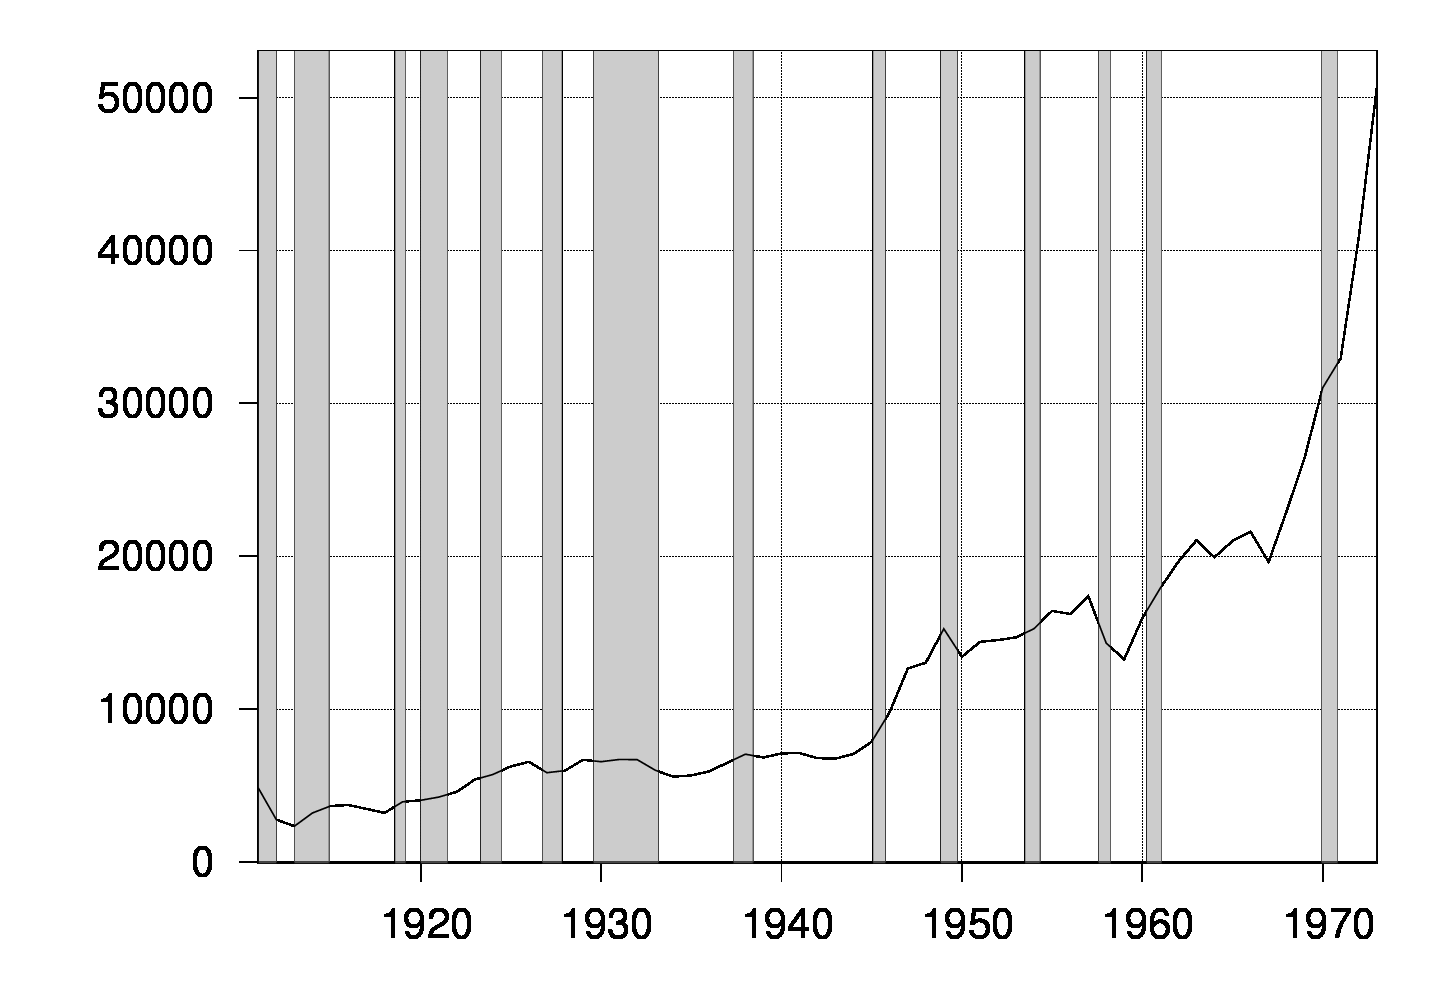
\includegraphics[scale=0.18]{avesals.png} \\
Panel (b): Log Average Nominal Salary \\
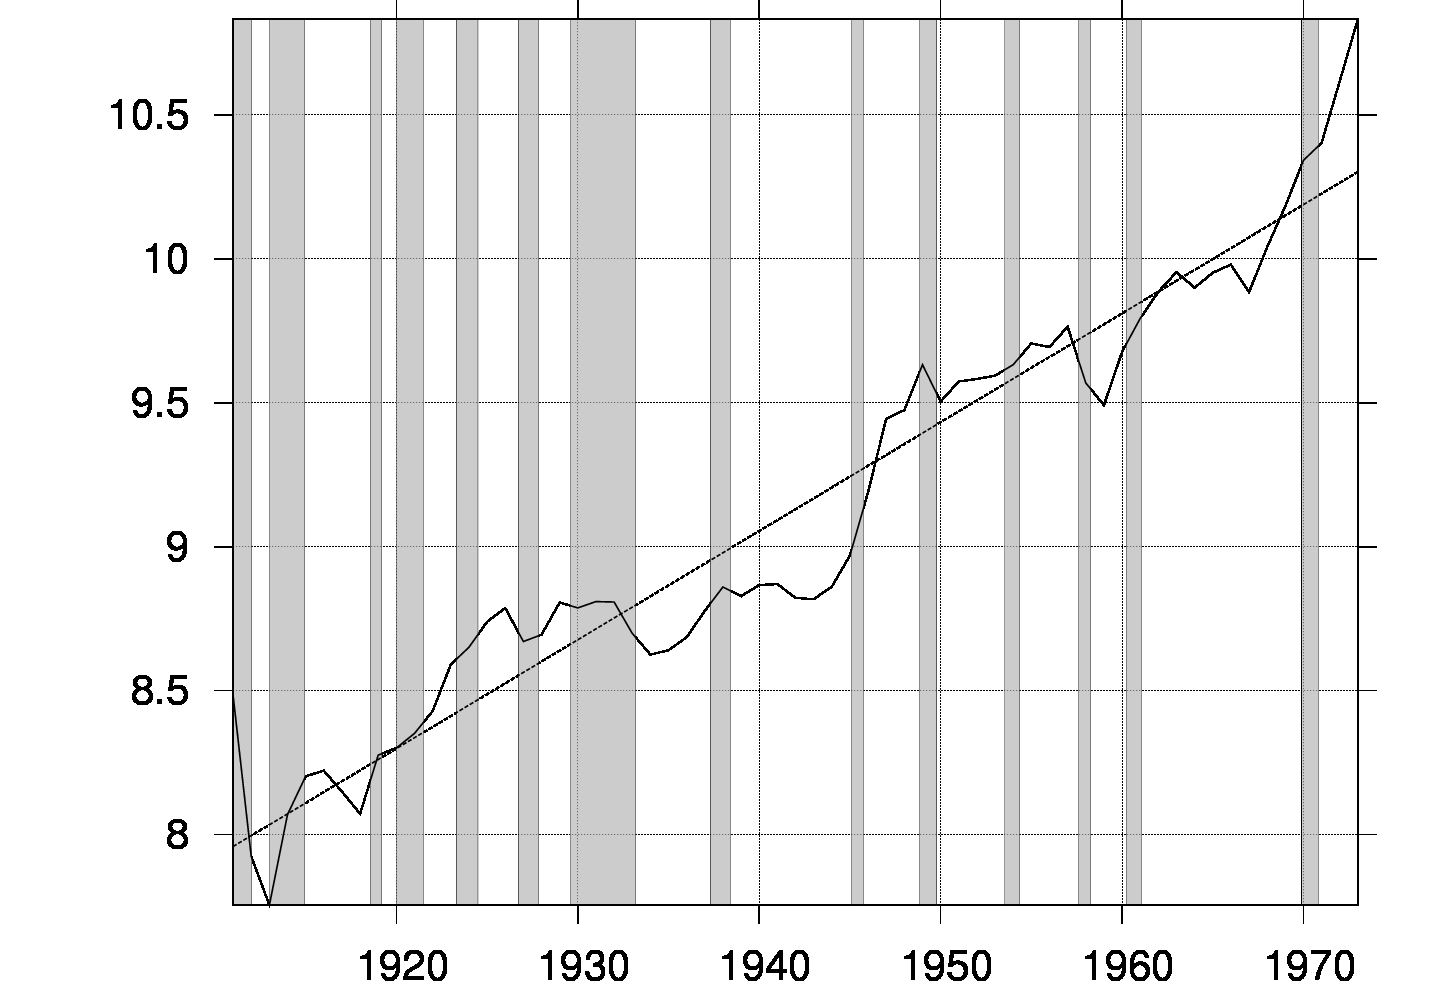
\includegraphics[scale=0.18]{logfitsals.png} \\
Panel (c): Deviation of Log Salary from Linear Trend \\
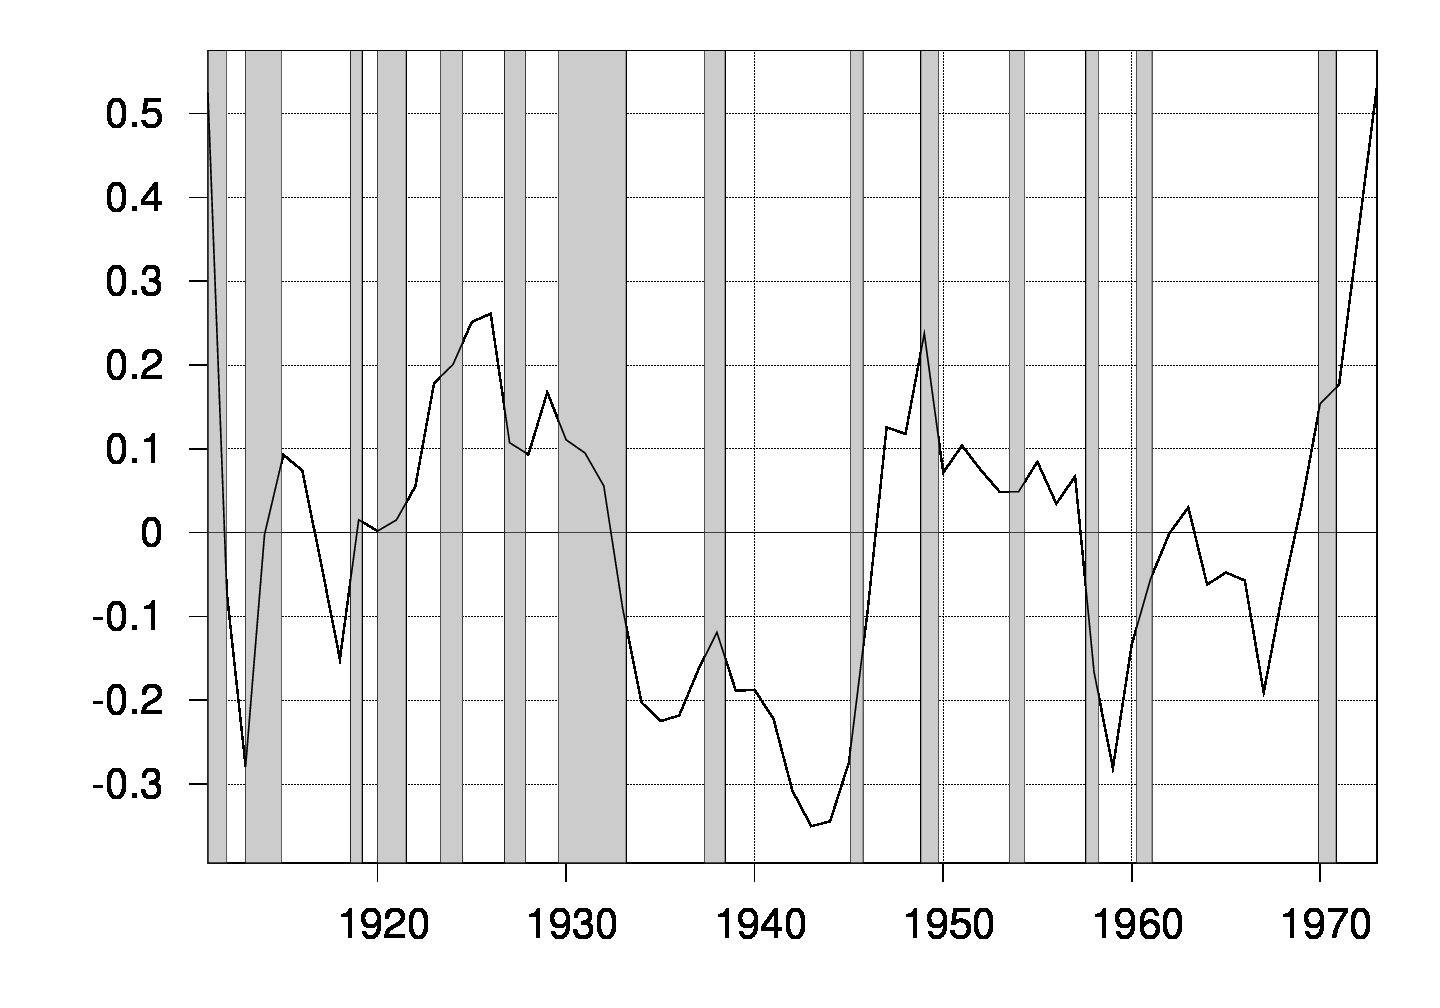
\includegraphics[scale=0.18]{salsres.png} 
\end{tabular}
\end{center}
\end{figure}

\begin{figure}\caption{Smoothed Probability the Labor Market is in Regime 2}\label{fg:regimes}
\begin{center}
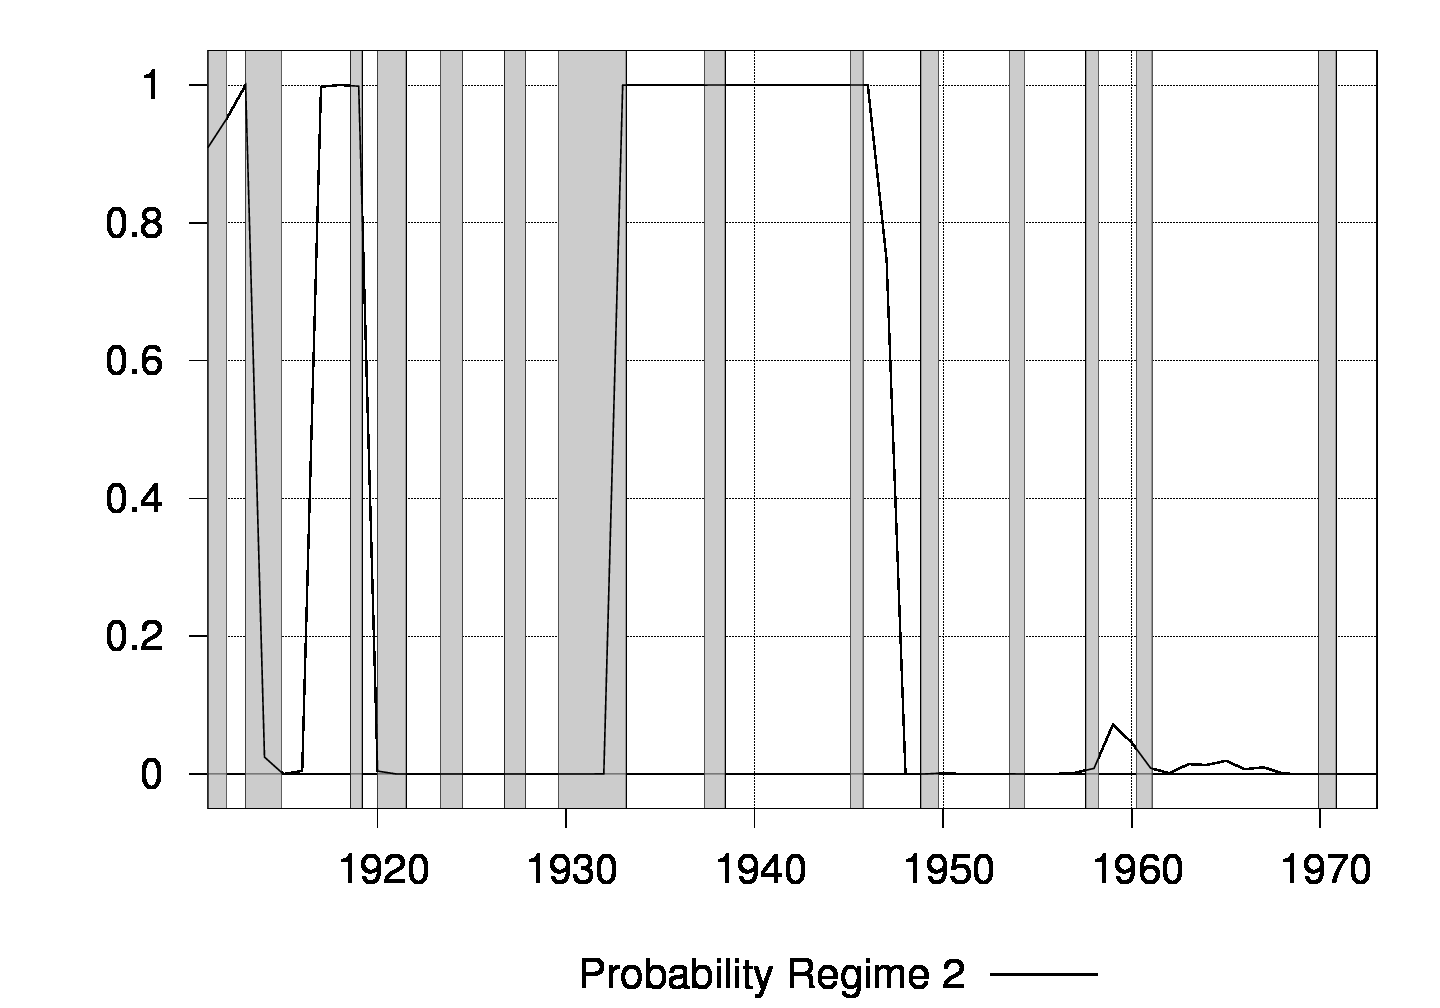
\includegraphics[scale=0.18]{regime.png} 
\end{center}
\end{figure}

\begin{table}\caption{Regime Switching Regression Results}\label{tb:results}
\begin{center}
\begin{tabular}{l|c|cc|c} 
 Variable & OLS & Regime 1 & Regime 2 & Difference \\ \hline 
 \multirow{2}{*}{Constant} & 4.5789*** & 4.0752*** & 5.0471*** & -0.9719** \\ 
 & (0.2314) & (0.2945) & (0.3401) & (0.4435) \\ [0.4pc]
 \multirow{2}{*}{Time} & 0.0325*** & 0.0320*** & 0.0323*** & -0.0004  \\ 
 & (0.0005) & (0.0006) & (0.0012) & (0.0014) \\ [0.4pc]
 \multirow{2}{*}{Age} & 0.1490*** & 0.1890*** & 0.1057*** & 0.0833*** \\ 
 & (0.0161) & (0.0207) & (0.0228) & (0.0305) \\ [0.4pc]
 \multirow{2}{*}{Age Squared} & -0.0025*** & -0.0030*** & -0.0018*** & -0.0012** \\ 
 & (0.0003) & (0.0004) & (0.0004) & (0.0005) \\ [0.4pc]
 \multirow{2}{*}{Experience} & 0.1054*** & 0.0992*** & 0.1082*** & -0.0090  \\ 
 & (0.0066) & (0.0089) & (0.0086) & (0.0123) \\ [0.4pc]
 \multirow{2}{*}{Experience Squared} & -0.0024*** & -0.0022*** & -0.0030*** & 0.0008  \\ 
 & (0.0004) & (0.0006) & (0.0005) & (0.0008) \\ [0.4pc]
 \multirow{2}{*}{Earned Run Average} & -0.0051** & -0.0023  & -0.0101*** & 0.0078* \\ 
 & (0.0024) & (0.0030) & (0.0037) & (0.0047) \\ [0.4pc]
 \multirow{2}{*}{Wins/Games} & 6.0445*** & 5.7505*** & 6.0059*** & -0.2555  \\ 
 & (0.2140) & (0.2863) & (0.3323) & (0.4021) \\ [0.4pc]
 \multirow{2}{*}{K/IP} & 0.3175*** & 0.1866*** & 0.4461*** & -0.2595*** \\ 
 & (0.0403) & (0.0511) & (0.0586) & (0.0762) \\ [0.4pc]\hline 
(Pseudo) $R^2$ & 0.8274 & \multicolumn{2}{c|}{0.8519} & - \\ 
Pseudo $R_{RS/OLS}^2$ & - & \multicolumn{2}{c|}{0.1418} & - \\ \hline
\multicolumn{5}{p{5in}}{\footnotesize{* Significant at 10\% level, ** Significant at 5\% level, *** Significant at 1\% level.\newline Standard errors in parentheses.  Number of observations = 2132,\newline Number of players = 403, Time period = 1911-1973.}}
\end{tabular}
\end{center}
\end{table}

\begin{table}\caption{Labor Market Regime Changes$^1$}\label{tb:regimes}
\begin{center}
\begin{tabular}{cc}
Time Period & Regime \\ \hline
1911-1913 & Regime 2 \\
1914-1916 & Regime 1 \\
1917-1919 & Regime 2 \\
1920-1932 & Regime 1 \\
1933-1947 & Regime 2 \\
1948-1973 & Regime 1 \\ \hline
\multicolumn{2}{p{2.5in}}{$^1$A time period is identified in a given regime if the smoothed probability is greater than 0.5.}
\end{tabular}
\end{center}
\end{table}






\end{document}


